\documentclass[11pt,a4paper]{article}

\usepackage[T1]{fontenc}
\usepackage[margin=2.5cm]{geometry}
\usepackage{lmodern}
\usepackage{microtype}
\usepackage{graphicx}
\usepackage{float}
\usepackage{fancyhdr}
\usepackage{tabularx}
\usepackage{array}
\usepackage{enumitem}
\usepackage{xcolor}
\usepackage{listings}
\usepackage{pgfgantt}
\usepackage{tikz}
\usetikzlibrary{positioning,shapes.geometric,shapes.multipart,arrows.meta,calc}
\usepackage[colorlinks=true,linkcolor=blue!50!black,urlcolor=blue!50!black]{hyperref}

\lstset{
  basicstyle=\ttfamily\footnotesize,
  keywordstyle=\color{blue!60!black},
  commentstyle=\color{green!40!black},
  stringstyle=\color{red!50!black},
  numbers=left, numberstyle=\tiny, frame=single,
  breaklines=true, language=Java, showstringspaces=false
}

% Boxed tables: slightly taller rows
\renewcommand{\arraystretch}{1.35}

\newcommand{\proj}{QR Code Based Attendance System}

\title{\proj}
\author{Md Jahidul Islam}
\date{\today}

\pagestyle{fancy}
\fancyhf{}
\lhead{\small Md Jahidul Islam (IT24018)}
\rhead{\small \proj}
\cfoot{\thepage}

\begin{document}

%==========================================================
% TITLE PAGE
%==========================================================
\begin{titlepage}
\centering
\vspace*{1.5cm}
{\LARGE\bfseries \proj\par}
\vspace{0.4cm}
{\large Final Capstone Project --- Part I: Proposal and Prototyping\par}
\vspace{1.5cm}

{\renewcommand{\arraystretch}{1.6}
\begin{tabular}{|p{4.2cm}|p{9cm}|}
\hline
\multicolumn{2}{|c|}{\textbf{Submission Details}}\\
\hline
\textbf{Submitted by} & Md Jahidul Islam\\ \hline
\textbf{Student ID} & IT24018\\ \hline
\textbf{Course} & Software Engineering and Project Management\\ \hline
\textbf{Department} & Information and Communication Technology\\ \hline
\textbf{University} & Mawlana Bhashani Science and Technology University\\ \hline
\textbf{Supervised by} & Dr. Ziaur Rahman\newline
Professor\newline
Dept. of ICT, MBSTU\\ \hline
\textbf{Date} & \today\\
\hline
\end{tabular}}

\vspace{1.5cm}
\textbf{Repository:}\\
\url{https://github.com/mohammadjahidulislam/smart-attendance-proposal}
\vfill
\end{titlepage}

\begin{abstract}
Manual and paper-based attendance in universities is slow, error-prone and hard to report on.
This proposal describes the \proj{}, a role-based system in which teachers open class sessions,
students check in, leave requests are submitted and approved online, and administrators receive
course-wise attendance reports. The system automatically warns students whose attendance falls
below a configurable threshold (default 75\%). The proposal covers the problem, scope,
requirements, risks, technology stack, budget, a Scrum-based schedule with a Gantt chart,
six UML diagrams, and a prototype built from five classes of the class diagram.
\end{abstract}

\tableofcontents
\newpage

%==========================================================
\section{Introduction}
\subsection{Background}
Universities must track student attendance for every course, because many institutions require a
minimum percentage for exam eligibility. Teachers still often use paper registers or spreadsheets,
which makes proxy attendance, calculation mistakes and delayed reporting common.

\subsection{Problem Statement}
\begin{itemize}[noitemsep]
  \item Taking attendance by roll call wastes class time.
  \item Calculating per-student attendance percentages by hand is slow and error-prone.
  \item Students learn about low attendance too late to act.
  \item Leave and medical excuses are handled on paper and are hard to verify.
  \item Administrators cannot easily get department or course-wise reports.
\end{itemize}

\subsection{Objectives}
\begin{enumerate}[noitemsep]
  \item Digitise attendance recording per class session.
  \item Compute attendance percentage per student per course automatically.
  \item Provide online leave application and approval.
  \item Send early warnings when attendance drops below the threshold.
  \item Provide exportable reports (CSV/PDF) for teachers and administrators.
\end{enumerate}

\subsection{Scope}
\textbf{In scope:} user management, course and session management, attendance marking,
leave management, low-attendance warnings, reports, admin dashboard.\\
\textbf{Out of scope:} biometric/face recognition, payroll, examination management, native mobile apps
(the web interface is responsive).

\subsection{Unique Features}
This project differs from a basic attendance recorder by focusing on (1) leave management with approval workflow,
(2) automatic low-attendance warnings and (3) an administrator reporting dashboard.

\subsection{Stakeholders}
\begin{tabularx}{\textwidth}{|l|X|}
\hline
\textbf{Stakeholder} & \textbf{Interest}\\
\hline
Student & Check in, view own attendance, apply for leave, receive warnings\\ \hline
Teacher & Open sessions, mark/correct attendance, approve leave, view course reports\\ \hline
Administrator & Manage users and courses, view dashboards and reports\\ \hline
Department head & Monitor attendance trends\\ \hline
Developer (Md Jahidul Islam) & Design, implement, test and document the system\\
\hline
\end{tabularx}

%==========================================================
\section{Requirements}
\subsection{Functional Requirements}
\begin{tabularx}{\textwidth}{|l|X|}
\hline
\textbf{ID} & \textbf{Requirement}\\
\hline
FR1 & Users shall log in with role-based access (Student, Teacher, Admin).\\ \hline
FR2 & Admin shall create and manage users, courses and enrolments.\\ \hline
FR3 & Teacher shall open and close a class session for a course.\\ \hline
FR4 & Student shall mark attendance while a session is open; teacher may correct records.\\ \hline
FR5 & System shall store status as Present, Absent, Late or Excused.\\ \hline
FR6 & Student shall submit a leave request with reason and dates.\\ \hline
FR7 & Teacher shall approve or reject leave; approved leave marks sessions as Excused.\\ \hline
FR8 & System shall compute attendance percentage per student per course.\\ \hline
FR9 & System shall notify students whose attendance is below the threshold.\\ \hline
FR10 & System shall export course and department reports as CSV and PDF.\\
\hline
\end{tabularx}

\subsection{Non-Functional Requirements}
\begin{tabularx}{\textwidth}{|l|X|}
\hline
\textbf{Attribute} & \textbf{Requirement}\\
\hline
Performance & Attendance marking shall complete within 2 seconds for up to 200 concurrent users.\\ \hline
Security & Passwords hashed; role-based authorization; HTTPS in deployment.\\ \hline
Usability & A new user shall mark attendance within 3 clicks after login.\\ \hline
Reliability & Availability of at least 99\% during working hours; daily database backup.\\ \hline
Maintainability & Layered architecture; unit-test coverage of at least 60\% for core classes.\\ \hline
Portability & Runs on modern browsers and on Windows/Linux servers.\\
\hline
\end{tabularx}

%==========================================================
\section{Feasibility and Risk Analysis}
\subsection{Feasibility}
\textbf{Technical:} uses mature open-source tools. \textbf{Economic:} low cost, no paid licences.
\textbf{Operational:} workflow mirrors the existing manual process. \textbf{Schedule:} 12 weeks, one developer.

\subsection{Risk Register}
\begin{tabularx}{\textwidth}{|l|X|c|c|X|}
\hline
\textbf{ID} & \textbf{Risk} & \textbf{Prob.} & \textbf{Impact} & \textbf{Mitigation}\\
\hline
R1 & Requirements change late & Med & High & Sprint reviews, prioritised backlog\\ \hline
R2 & Single developer unavailable (illness) & Low & High & Buffer in each sprint, daily commits\\ \hline
R3 & Proxy attendance by students & High & Med & Time-limited sessions, teacher correction, audit log\\ \hline
R4 & Data loss & Low & High & Daily backups, version control\\ \hline
R5 & Underestimated effort & Med & Med & Re-estimate each sprint, cut low-priority features\\ \hline
R6 & Security breach / weak passwords & Low & High & Hashing, input validation, role checks\\
\hline
\end{tabularx}

%==========================================================
\section{Technology Stack, Resources and Budget}
\begin{tabularx}{\textwidth}{|l|X|}
\hline
\textbf{Layer} & \textbf{Choice}\\
\hline
Language & Java 17\\ \hline
Backend / Web & Javalin (REST API)\\ \hline
Database & SQLite for prototype; MySQL/PostgreSQL for deployment\\ \hline
Frontend & HTML, CSS, JavaScript (responsive); JavaFX for the desktop prototype\\ \hline
Build & Maven\\ \hline
Testing & JUnit 5\\ \hline
Version control & Git and GitHub\\ \hline
Documentation & \LaTeX{}, PlantUML/TikZ\\
\hline
\end{tabularx}

\subsection{Estimated Budget}
\begin{tabularx}{\textwidth}{|X|r|}
\hline
\textbf{Item} & \textbf{Cost (BDT)}\\
\hline
Developer effort (12 weeks, academic project) & 0\\ \hline
Development laptop (existing) & 0\\ \hline
Cloud hosting / domain (optional, 3 months) & 3{,}000\\ \hline
Internet and miscellaneous & 2{,}000\\ \hline
Contingency (10\%) & 500\\ \hline
\textbf{Total} & \textbf{5{,}500}\\
\hline
\end{tabularx}

%==========================================================
\section{Software Process Model and Schedule}
\subsection{Chosen Model: Agile (Scrum)}
Scrum is used because requirements (reports, notifications) are likely to evolve and the
product can be delivered incrementally. Work is organised into six two-week sprints.
Each sprint ends with a working increment, a review and a retrospective. The product backlog is kept
in GitHub Projects.

\subsection{Sprint Plan}
\begin{tabularx}{\textwidth}{|l|l|X|}
\hline
\textbf{Sprint} & \textbf{Dates (2026--27)} & \textbf{Goal and deliverable}\\
\hline
1 & 2 Nov -- 15 Nov & Requirements, backlog, proposal document\\ \hline
2 & 16 Nov -- 29 Nov & UML design, database schema, UI wireframes\\ \hline
3 & 30 Nov -- 13 Dec & Login, users, courses, sessions, attendance marking\\ \hline
4 & 14 Dec -- 27 Dec & Leave management and approval workflow\\ \hline
5 & 28 Dec -- 10 Jan & Percentage calculation, warnings, reports (CSV/PDF)\\ \hline
6 & 11 Jan -- 24 Jan & Testing, bug fixing, deployment, final documentation\\
\hline
\end{tabularx}

\subsection{Milestones and Deliverables}
\begin{tabularx}{\textwidth}{|l|l|X|}
\hline
\textbf{ID} & \textbf{Week} & \textbf{Milestone / Deliverable}\\
\hline
M1 & 2 & Approved proposal and product backlog\\ \hline
M2 & 4 & UML diagrams and database design complete\\ \hline
M3 & 6 & Attendance module working (demo)\\ \hline
M4 & 8 & Leave management working\\ \hline
M5 & 10 & Reports and warnings working\\ \hline
M6 & 12 & Tested system, user manual, final report\\
\hline
\end{tabularx}

\subsection{Gantt Chart}
\begin{figure}[H]
\centering
\resizebox{\textwidth}{!}{%
\begin{ganttchart}[
  vgrid, hgrid,
  x unit=0.75cm, y unit title=0.6cm, y unit chart=0.65cm,
  bar/.append style={fill=blue!45},
  milestone/.append style={fill=red!70},
  title label font=\footnotesize, bar label font=\footnotesize
]{1}{12}
\gantttitle{Week}{12}\\
\gantttitlelist{1,...,12}{1}\\
\ganttbar{Requirements}{1}{2}\\
\ganttbar{Design (UML, DB, UI)}{3}{4}\\
\ganttbar{Attendance module}{5}{6}\\
\ganttbar{Leave management}{7}{8}\\
\ganttbar{Reports and warnings}{9}{10}\\
\ganttbar{Testing and deployment}{11}{12}\\
\ganttbar{Documentation}{1}{12}\\
\ganttmilestone{Milestones M1--M6}{2}\ganttmilestone{}{4}\ganttmilestone{}{6}
\ganttmilestone{}{8}\ganttmilestone{}{10}\ganttmilestone{}{12}
\end{ganttchart}}
\caption{Project Gantt chart (12 weeks, starting 2 November 2026).}
\end{figure}

%==========================================================
\section{System Design (UML Diagrams)}

\subsection{Data Flow Diagram}
\tikzset{
  ent/.style={rectangle,draw,minimum width=2.2cm,minimum height=0.9cm,font=\small},
  proc/.style={circle,draw,align=center,font=\scriptsize,inner sep=2pt,text width=2.1cm},
  store/.style={draw=none,minimum width=3cm,minimum height=0.8cm,font=\scriptsize,
    append after command={\pgfextra{
      \draw (\tikzlastnode.north west)--(\tikzlastnode.north east);
      \draw (\tikzlastnode.south west)--(\tikzlastnode.south east);}}},
  flow/.style={-{Stealth[length=2mm]}}
}

\subsubsection*{Level 0 (context diagram).}
\begin{figure}[H]
\centering
\resizebox{0.95\textwidth}{!}{%
\begin{tikzpicture}
\node[proc,text width=2.8cm] (p) at (6,0) {\textbf{0}\\Smart Attendance\\System};
\node[ent] (stu) at (0,3) {Student};
\node[ent] (tea) at (0,-3) {Teacher};
\node[ent] (adm) at (12,0) {Administrator};
\draw[flow] (stu) to[bend left=15] node[above,sloped,font=\tiny]{login, check-in, leave request} (p);
\draw[flow] (p) to[bend left=15] node[below,sloped,font=\tiny]{attendance \%, warnings} (stu);
\draw[flow] (tea) to[bend left=15] node[above,sloped,font=\tiny]{open session, corrections, leave decision} (p);
\draw[flow] (p) to[bend left=15] node[below,sloped,font=\tiny]{course reports, leave requests} (tea);
\draw[flow] (adm) to[bend left=15] node[above,sloped,font=\tiny]{users, courses} (p);
\draw[flow] (p) to[bend left=15] node[below,sloped,font=\tiny]{dashboard, reports} (adm);
\end{tikzpicture}}
\caption{DFD Level 0.}
\end{figure}

\subsubsection*{Level 1.}
\begin{figure}[H]
\centering
\resizebox{\textwidth}{!}{%
\begin{tikzpicture}
\node[ent] (e1) at (0,3) {Student};
\node[ent] (e2) at (0,0.5) {Teacher};
\node[ent] (e3) at (0,-2) {Student / Teacher};
\node[ent] (e4) at (0,-4.5) {Administrator};
\node[proc] (p1) at (5,3) {\textbf{1.0}\\Mark Attendance};
\node[proc] (p2) at (5,0.5) {\textbf{2.0}\\Manage Sessions};
\node[proc] (p3) at (5,-2) {\textbf{3.0}\\Process Leave};
\node[proc] (p4) at (5,-4.5) {\textbf{4.0}\\Reports and Warnings};
\node[store] (d1) at (10.5,3) {D1 Attendance};
\node[store] (d2) at (10.5,0.5) {D2 Sessions};
\node[store] (d3) at (10.5,-2) {D3 Leave Requests};
\node[store] (d4) at (10.5,-4.5) {D4 All Records};
\draw[flow] (e1) -- node[above,font=\tiny]{check-in} (p1);
\draw[flow] (e2) -- node[above,font=\tiny]{open/close} (p2);
\draw[flow] (e3) -- node[above,font=\tiny]{apply/decide} (p3);
\draw[flow] (e4) -- node[above,font=\tiny]{report request} (p4);
\draw[flow] (p1) -- (d1);
\draw[flow] (p2) -- (d2);
\draw[flow] (p3) -- (d3);
\draw[flow] (d4) -- (p4);
\end{tikzpicture}}
\caption{DFD Level 1.}
\end{figure}

%----------------------------------------------------------
\subsection{Use Case Diagram}
\begin{figure}[H]
\centering
\resizebox{0.85\textwidth}{!}{%
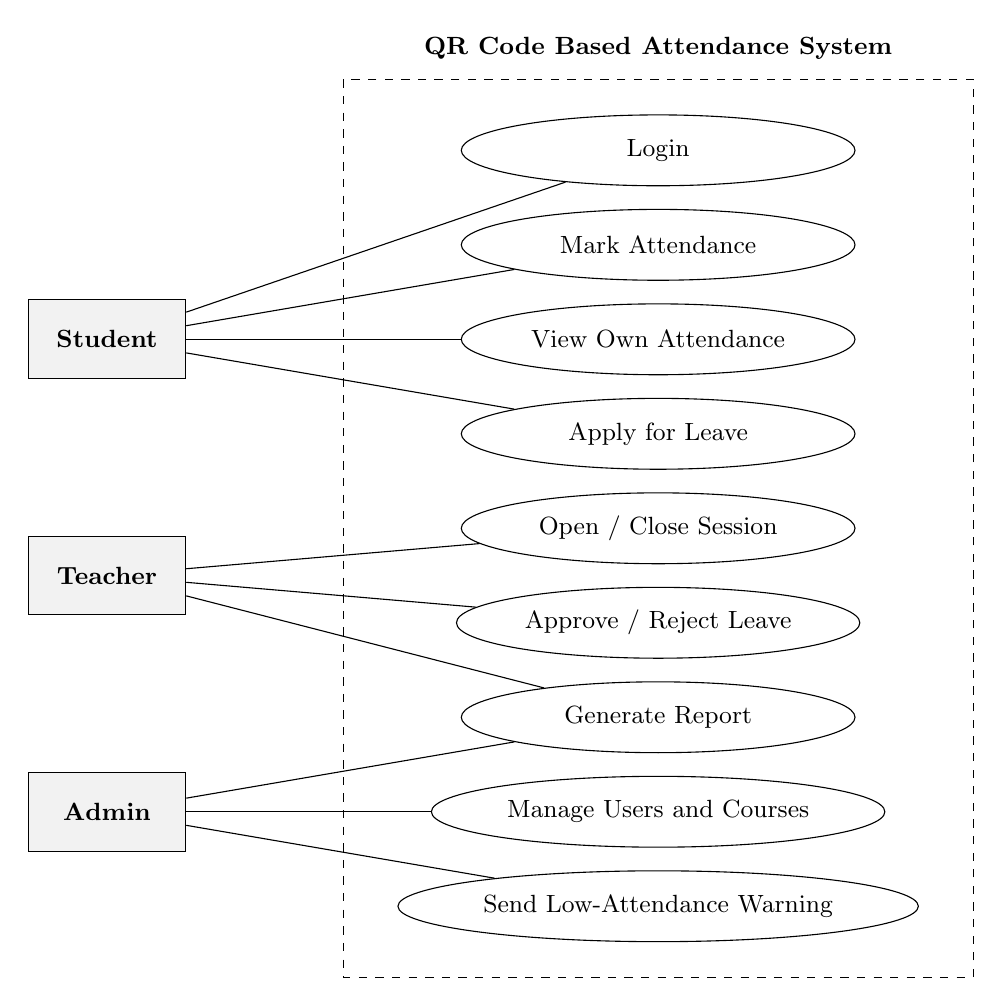
\begin{tikzpicture}
\tikzset{uc/.style={ellipse,draw,minimum width=5cm,minimum height=0.9cm,font=\small},
         act/.style={rectangle,draw,minimum width=2cm,minimum height=1cm,font=\small\bfseries,fill=gray!10}}
\draw[dashed] (3,0.9) rectangle (11,-10.5);
\node[font=\small\bfseries] at (7,1.3) {\proj};
\node[uc] (u1) at (7,0) {Login};
\node[uc] (u2) at (7,-1.2) {Mark Attendance};
\node[uc] (u3) at (7,-2.4) {View Own Attendance};
\node[uc] (u4) at (7,-3.6) {Apply for Leave};
\node[uc] (u5) at (7,-4.8) {Open / Close Session};
\node[uc] (u6) at (7,-6.0) {Approve / Reject Leave};
\node[uc] (u7) at (7,-7.2) {Generate Report};
\node[uc] (u8) at (7,-8.4) {Manage Users and Courses};
\node[uc] (u9) at (7,-9.6) {Send Low-Attendance Warning};
\node[act] (s) at (0,-2.4) {Student};
\node[act] (t) at (0,-5.4) {Teacher};
\node[act] (a) at (0,-8.4) {Admin};
\draw (s) -- (u1); \draw (s) -- (u2); \draw (s) -- (u3); \draw (s) -- (u4);
\draw (t) -- (u5); \draw (t) -- (u6); \draw (t) -- (u7);
\draw (a) -- (u7); \draw (a) -- (u8); \draw (a) -- (u9);
\end{tikzpicture}}
\caption{Use case diagram (all actors log in first).}
\end{figure}

%----------------------------------------------------------
\subsection{Activity Diagram}
\begin{figure}[H]
\centering
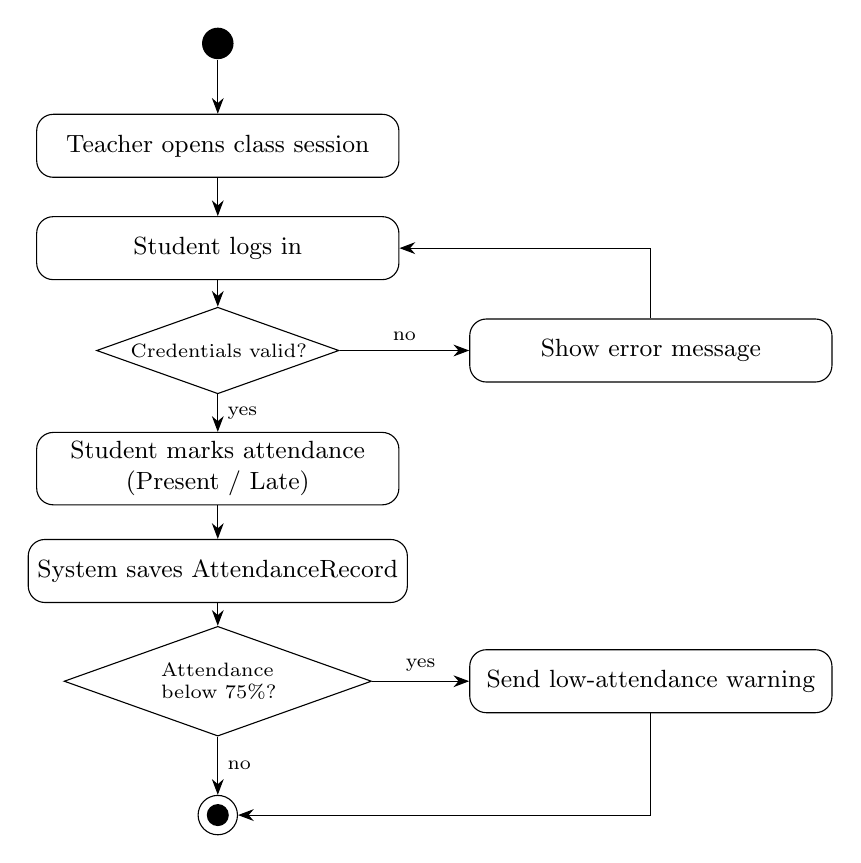
\begin{tikzpicture}[
  act/.style={rectangle,rounded corners=6pt,draw,minimum width=4.6cm,minimum height=0.8cm,font=\small,align=center},
  dec/.style={diamond,aspect=2.8,draw,font=\scriptsize,align=center,inner sep=0pt,text width=2.6cm},
  flow/.style={-{Stealth[length=2mm]}}]
\node[circle,fill=black,minimum size=0.4cm] (st) at (0,0) {};
\node[act] (a1) at (0,-1.3) {Teacher opens class session};
\node[act] (a2) at (0,-2.6) {Student logs in};
\node[dec] (d1) at (0,-3.9) {Credentials valid?};
\node[act] (er) at (5.5,-3.9) {Show error message};
\node[act] (a3) at (0,-5.4) {Student marks attendance\\(Present / Late)};
\node[act] (a4) at (0,-6.7) {System saves AttendanceRecord};
\node[dec] (d2) at (0,-8.1) {Attendance below 75\%?};
\node[act] (a5) at (5.5,-8.1) {Send low-attendance warning};
\node[circle,draw,minimum size=0.5cm,inner sep=1pt] (en) at (0,-9.8) {\tikz\fill (0,0) circle (0.14cm);};
\draw[flow] (st)--(a1); \draw[flow] (a1)--(a2); \draw[flow] (a2)--(d1);
\draw[flow] (d1)--node[right,font=\scriptsize]{yes}(a3);
\draw[flow] (d1)--node[above,font=\scriptsize]{no}(er);
\draw[flow] (er.north) |- (a2.east);
\draw[flow] (a3)--(a4); \draw[flow] (a4)--(d2);
\draw[flow] (d2)--node[above,font=\scriptsize]{yes}(a5);
\draw[flow] (d2)--node[right,font=\scriptsize]{no}(en);
\draw[flow] (a5.south) |- (en.east);
\end{tikzpicture}
\caption{Activity diagram: marking attendance and low-attendance warning.}
\end{figure}

%----------------------------------------------------------
\subsection{Entity Relationship Diagram}
\begin{figure}[H]
\centering
\resizebox{\textwidth}{!}{%
\begin{tikzpicture}
\tikzset{ent/.style={rectangle,draw,minimum width=2.6cm,minimum height=0.9cm,font=\small\bfseries},
         rel/.style={diamond,draw,aspect=2,inner sep=1pt,font=\scriptsize}}
\newcommand{\card}[4]{\draw (#1) -- (#2) node[pos=#3,fill=white,inner sep=1pt,font=\scriptsize]{#4};}
\node[ent] (tea) at (0,0) {Teacher};
\node[rel] (con) at (3.2,0) {Conducts};
\node[ent] (ses) at (6.4,0) {ClassSession};
\node[rel] (has) at (9.6,0) {Has};
\node[ent] (crs) at (12.8,0) {Course};
\node[rel] (enr) at (12.8,-2.3) {Enrolls};
\node[ent] (stu) at (12.8,-4.6) {Student};
\node[rel] (mar) at (9.6,-4.6) {Marked by};
\node[ent] (att) at (6.4,-4.6) {Attendance};
\node[rel] (for) at (6.4,-2.3) {Recorded in};
\node[rel] (app) at (12.8,-6.9) {Applies};
\node[ent] (lea) at (12.8,-9.2) {LeaveRequest};
\card{tea}{con}{0.15}{1}\card{con}{ses}{0.85}{N}
\card{ses}{has}{0.15}{N}\card{has}{crs}{0.85}{1}
\card{crs}{enr}{0.15}{M}\card{enr}{stu}{0.85}{N}
\card{stu}{mar}{0.15}{1}\card{mar}{att}{0.85}{N}
\card{ses}{for}{0.15}{1}\card{for}{att}{0.85}{N}
\card{stu}{app}{0.15}{1}\card{app}{lea}{0.85}{N}
\end{tikzpicture}}
\caption{ER diagram (cardinalities shown on the lines).}
\end{figure}

\subsubsection*{Attributes.}
\begin{tabularx}{\textwidth}{|l|X|}
\hline
\textbf{Entity} & \textbf{Attributes (primary key in italics)}\\
\hline
Student & \textit{studentId}, name, department, email, passwordHash\\ \hline
Teacher & \textit{teacherId}, name, email, passwordHash\\ \hline
Course & \textit{courseCode}, title, credit, teacherId (FK)\\ \hline
ClassSession & \textit{sessionId}, courseCode (FK), teacherId (FK), date, startTime, room, isOpen\\ \hline
Attendance & \textit{attendanceId}, studentId (FK), sessionId (FK), status, markedAt\\ \hline
LeaveRequest & \textit{leaveId}, studentId (FK), fromDate, toDate, reason, status, approvedBy\\
\hline
\end{tabularx}

%----------------------------------------------------------
\subsection{Class Diagram}
\begin{figure}[H]
\centering
\resizebox{\textwidth}{!}{%
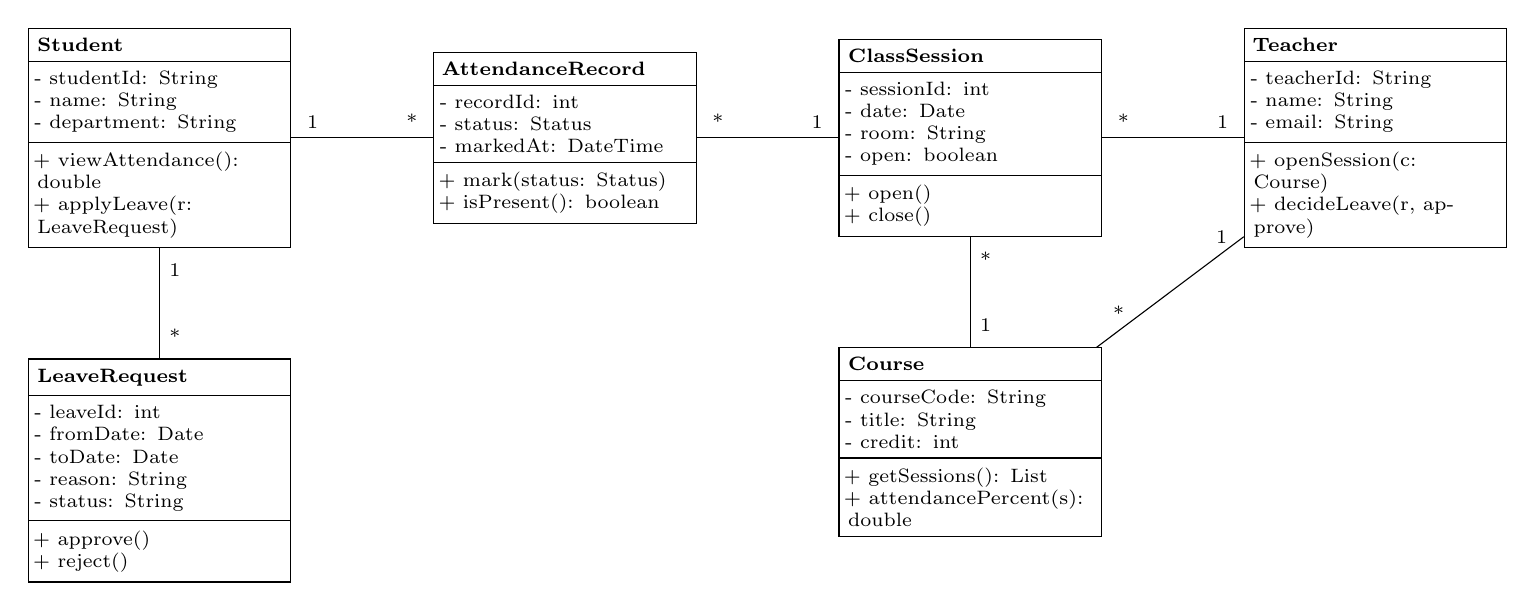
\begin{tikzpicture}[
  class/.style={rectangle split,rectangle split parts=3,draw,font=\scriptsize,
    text width=3.1cm,align=left,rectangle split part align={center,left,left}},
  node distance=1.4cm and 1.8cm]
\node[class] (stu) {\textbf{Student}\nodepart{second}- studentId: String\\- name: String\\- department: String\nodepart{third}+ viewAttendance(): double\\+ applyLeave(r: LeaveRequest)};
\node[class,right=of stu] (att) {\textbf{AttendanceRecord}\nodepart{second}- recordId: int\\- status: Status\\- markedAt: DateTime\nodepart{third}+ mark(status: Status)\\+ isPresent(): boolean};
\node[class,right=of att] (ses) {\textbf{ClassSession}\nodepart{second}- sessionId: int\\- date: Date\\- room: String\\- open: boolean\nodepart{third}+ open()\\+ close()};
\node[class,right=of ses] (tea) {\textbf{Teacher}\nodepart{second}- teacherId: String\\- name: String\\- email: String\nodepart{third}+ openSession(c: Course)\\+ decideLeave(r, approve)};
\node[class,below=of stu] (lea) {\textbf{LeaveRequest}\nodepart{second}- leaveId: int\\- fromDate: Date\\- toDate: Date\\- reason: String\\- status: String\nodepart{third}+ approve()\\+ reject()};
\node[class,below=of ses] (crs) {\textbf{Course}\nodepart{second}- courseCode: String\\- title: String\\- credit: int\nodepart{third}+ getSessions(): List\\+ attendancePercent(s): double};
\draw (stu) -- node[pos=0.15,above,font=\scriptsize]{1} node[pos=0.85,above,font=\scriptsize]{*} (att);
\draw (ses) -- node[pos=0.15,above,font=\scriptsize]{1} node[pos=0.85,above,font=\scriptsize]{*} (att);
\draw (tea) -- node[pos=0.15,above,font=\scriptsize]{1} node[pos=0.85,above,font=\scriptsize]{*} (ses);
\draw (crs) -- node[pos=0.2,right,font=\scriptsize]{1} node[pos=0.8,right,font=\scriptsize]{*} (ses);
\draw (stu) -- node[pos=0.2,right,font=\scriptsize]{1} node[pos=0.8,right,font=\scriptsize]{*} (lea);
\draw (tea) -- node[pos=0.15,above,font=\scriptsize]{1} node[pos=0.85,above,font=\scriptsize]{*} (crs);
\end{tikzpicture}}
\caption{Class diagram. Associations: Student--AttendanceRecord, ClassSession--AttendanceRecord, Teacher--ClassSession, Course--ClassSession, Student--LeaveRequest, Teacher--Course.}
\end{figure}

%----------------------------------------------------------
\subsection{Object Diagram}
\begin{figure}[H]
\centering
\resizebox{\textwidth}{!}{%
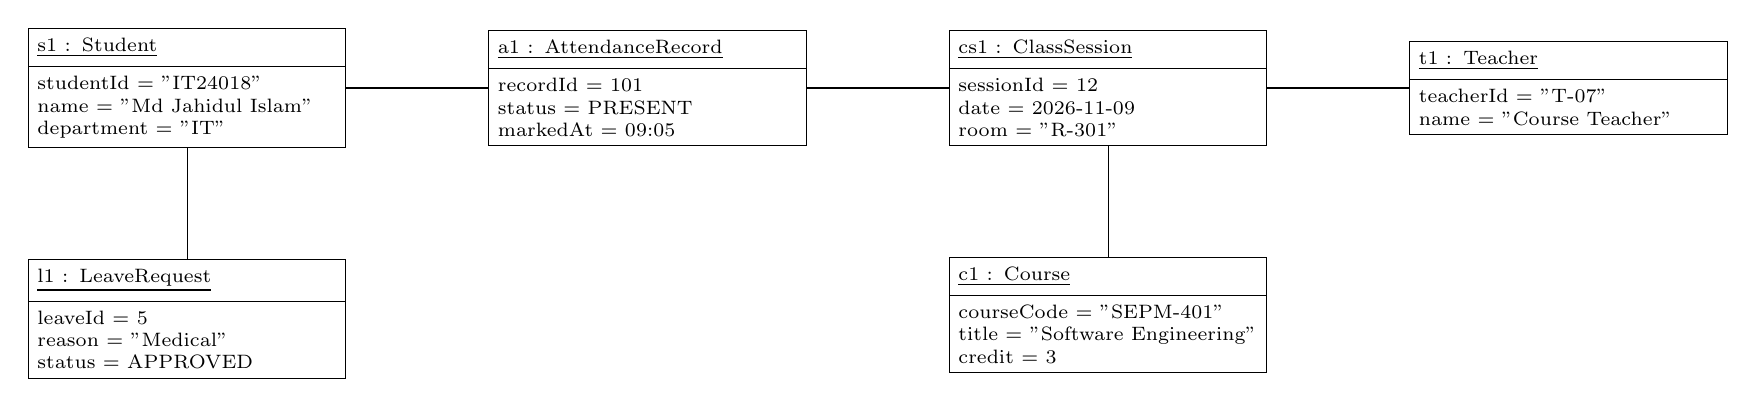
\begin{tikzpicture}[
  obj/.style={rectangle split,rectangle split parts=2,draw,font=\scriptsize,text width=3.8cm,align=left,
    rectangle split part align={center,left}},
  node distance=1.4cm and 1.8cm]
\node[obj] (s1) {\underline{s1 : Student}\nodepart{second}studentId = "IT24018"\\name = "Md Jahidul Islam"\\department = "IT"};
\node[obj,right=of s1] (a1) {\underline{a1 : AttendanceRecord}\nodepart{second}recordId = 101\\status = PRESENT\\markedAt = 09:05};
\node[obj,right=of a1] (cs1) {\underline{cs1 : ClassSession}\nodepart{second}sessionId = 12\\date = 2026-11-09\\room = "R-301"};
\node[obj,below=of cs1] (c1) {\underline{c1 : Course}\nodepart{second}courseCode = "SEPM-401"\\title = "Software Engineering"\\credit = 3};
\node[obj,right=of cs1] (t1) {\underline{t1 : Teacher}\nodepart{second}teacherId = "T-07"\\name = "Course Teacher"};
\node[obj,below=of s1] (l1) {\underline{l1 : LeaveRequest}\nodepart{second}leaveId = 5\\reason = "Medical"\\status = APPROVED};
\draw (s1) -- (a1); \draw (a1) -- (cs1); \draw (cs1) -- (t1);
\draw (c1) -- (cs1); \draw (s1) -- (l1);
\end{tikzpicture}}
\caption{Object diagram: one snapshot of the running system (sample values).}
\end{figure}

%==========================================================
\clearpage
\section{Prototype}
The prototype is a simple interface (JavaFX desktop or Javalin web page) built on five classes of the class diagram:
\texttt{Student}, \texttt{Teacher}, \texttt{Course}, \texttt{ClassSession} and \texttt{AttendanceRecord}.
\texttt{LeaveRequest} is added in Sprint 4.

\begin{tabularx}{\textwidth}{|l|X|}
\hline
\textbf{Class} & \textbf{Role in prototype}\\
\hline
Student & Logs in, marks attendance, sees own percentage\\ \hline
Teacher & Opens/closes a session, sees the attendance list\\ \hline
Course & Groups sessions and computes course attendance\\ \hline
ClassSession & Represents one class meeting, open or closed\\ \hline
AttendanceRecord & Stores one student's status for one session\\
\hline
\end{tabularx}

\subsubsection*{Core class (excerpt).}
\begin{lstlisting}
public class AttendanceRecord {
    public enum Status { PRESENT, ABSENT, LATE, EXCUSED }

    private final Student student;
    private final ClassSession session;
    private Status status;

    public AttendanceRecord(Student student, ClassSession session, Status status) {
        if (!session.isOpen()) throw new IllegalStateException("Session is closed");
        this.student = student;
        this.session = session;
        this.status = status;
    }

    public boolean isPresent() {
        return status == Status.PRESENT || status == Status.LATE;
    }
}
\end{lstlisting}

\subsubsection*{Interface screenshot.}
\begin{figure}[H]
\centering
\IfFileExists{screenshots/ui.png}{\includegraphics[width=0.8\textwidth]{screenshots/ui.png}}{%
\fbox{\parbox{0.8\textwidth}{\centering\vspace{3cm}Place the prototype screenshot at \texttt{screenshots/ui.png}\vspace{3cm}}}}
\caption{Prototype interface.}
\end{figure}

\subsubsection*{Repository structure.}
\begin{lstlisting}[language={},numbers=none]
smart-attendance-proposal/
  proposal.tex          (this document)
  screenshots/ui.png
  diagrams/             (UML source files)
  prototype/
    src/main/java/    (Student, Teacher, Course, ClassSession, AttendanceRecord, Main)
    pom.xml
  README.md
\end{lstlisting}

%==========================================================
\section{Testing and Quality Plan}
\begin{itemize}[noitemsep]
  \item \textbf{Unit tests} (JUnit 5) for percentage calculation, session open/close rules and leave approval.
  \item \textbf{Integration tests} for the REST endpoints and database access.
  \item \textbf{User acceptance test} with at least five classmates acting as students and one as teacher.
  \item \textbf{Quality practices:} code review via pull requests, one feature per branch, sprint retrospectives.
\end{itemize}

\section{Conclusion}
The \proj{} reduces class time spent on roll call, removes manual percentage calculation, gives students early
warnings and gives administrators reliable reports. The Scrum plan delivers a working increment every two weeks,
and the prototype demonstrates the core classes defined in the UML design.

\begin{thebibliography}{9}
\bibitem{sommerville} I. Sommerville, \textit{Software Engineering}, 10th ed., Pearson, 2016.
\bibitem{pressman} R. S. Pressman, \textit{Software Engineering: A Practitioner's Approach}, McGraw-Hill.
\bibitem{scrum} K. Schwaber and J. Sutherland, \textit{The Scrum Guide}, 2020.
\bibitem{uml} OMG, \textit{Unified Modeling Language Specification}, v2.5.1.
\end{thebibliography}

\end{document}
